\documentclass{article}
\usepackage{graphicx}
\usepackage[center]{caption}
\usepackage{float}
\graphicspath{ {./img} }
\title{Diplomarbeit: App für Menschen in Not}
\date{15.06.2022}
\author{Jakob Holzinger, Jonas Denk}
\begin{document}
\maketitle
\frenchspacing
\raggedbottom
\pagestyle{plain}
\section{Informationen zu unserer Diplomarbeit}
Die Idee hinter der App ist es, dass Menschen in Not per Knopfdruck auf sich aufmerksam machen können und schnellstmöglich durch das Kollektiv der anderen App User Hilfe bekommen.
Wir arbeiten mit der Firma BizzNetIT zusammen. Jonas arbeitet dort.
\section{Arbeitsaufteilung}
\section{Konzept}
\subsection{Authentifizierung}
Prinzipiell gibt es zwei Arten von Usern. Den Security-User (Personal der Security-Firma) und den normalen User (Personen, welche die App besitzen). Es wird daher zwei Arten von Log-in's geben, einmal den Login wo sich die Securities einloggen und den wo sich die normalen User anmelden. 
\begin{figure}[H] 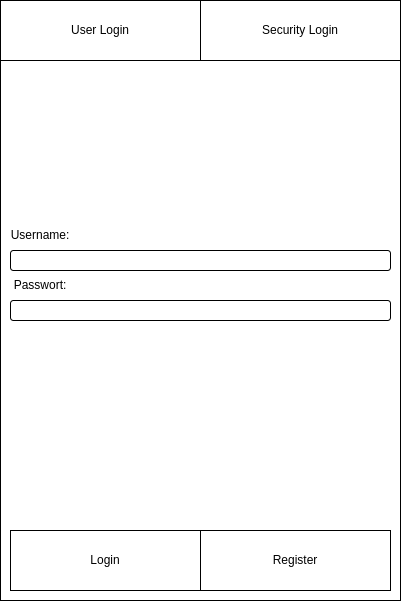
\includegraphics[scale=0.75]{login} \centering \caption{Log-in Screen} \end{figure}
\subsection{Datenbankzugriff}
Wir benötigen für den Authentifizierungsprozess natürlich eine Datenbank. In dieser werden die Anmeldedaten der User gespeichert.
\subsection{Was passiert wenn jemand den Notfall Knopf drückt?}
Wenn ein User in der App den Panic-Button auslöst wird ein Signal ausgesendet, dass der User Hilfe benötigt. 
Die App schaut im Umkreis nach, ob Security Mitarbeiter aufzufinden sind. 
Falls ja, wird an diese eine Benachrichtigung mit dem Ort des Users, welcher den Alarm ausgelöst hat, gesendet. 
Es wird dem Security Mitarbeiter ebenfalls, der schnellste Weg zum Opfer, in der App gezeigt (per Google Maps implementation). 
Wird kein Mitarbeiter im näheren Umkreis (ca. 2km) gefunden, geht die Benachrichtigung an alle User der App raus. Falls sich im näheren Umkreis keine User finden lassen wird die Umkreissuche so lange erweitert, bis User benachrichtigt werden. 
Wenn ein User den Notfallknopf betätigt wird automatisch das GPS auf seinem Gerät aktiviert, um den Helfenden die Möglichkeit zu geben den Alarmierenden zu finden.
\subsection{Dokumentation und Versionsverwaltung}
Dokumentiert wird bei uns ausschließlich in LaTex. 
Alle Referenzen werden in einem gemeinsam genutzten bibliography-file gespeichert.
Als Versionsverwaltung verwenden wir git. Unser Repository ist zu finden unter: INSERT LINK
\end{document}
